\documentclass{article}

\usepackage[utf8]{inputenc}
\usepackage[german]{babel}
\usepackage{amsmath}
\usepackage{csquotes}
\usepackage{booktabs}
\usepackage{graphicx}


\title{Erste Notizen für Vortrag 06.11.2024}
\author{David Antony}
\date{\today}

% This "\code{my code}" can be used to highlight small code snippets in the text like names of variables or methods.
\usepackage{multirow}
\newcommand{\code}[1]{\textcolor{black}{\texttt{#1}}}
% multirow with shortstack to allow line breaks
\newcommand{\cell}[1]{
	\multirow{2}{*}{\shortstack[l]{#1}}
}

% multirow with more control
\newcommand{\mcell}[3]{\multirow{#1}{*}{\shortstack[#2]{#3}}}
\newcommand{\todo}[1]{\textcolor{red}{\textbf{TODO:} #1}}
\newcommand{\note}[1]{\textcolor{blue}{\textbf{Note:} #1}}
\newcommand{\important}[1]{\textcolor{green}{\textbf{Important:} #1}}
\newcommand{\highlight}[1]{\colorbox{yellow}{#1}}
\newcommand{\email}[1]{\href{mailto:#1}{\texttt{#1}}}

\newcommand{\gl}{\glqq}
\newcommand{\gr}{\grqq\ }
\newcommand{\ul}[1]{\underline{#1}}


\makeatletter
\newsavebox\myboxA
\newsavebox\myboxB
\newlength\mylenA
\newcommand*\xoverline[2][0.75]{%
	\sbox{\myboxA}{$\m@th#2$}%
	\setbox\myboxB\null% Phantom box
	\ht\myboxB=\ht\myboxA%
	\dp\myboxB=\dp\myboxA%
	\wd\myboxB=#1\wd\myboxA% Scale phantom
	\sbox\myboxB{$\m@th\overline{\copy\myboxB}$}%  Overlined phantom
	\setlength\mylenA{\the\wd\myboxA}%   calc width diff
	\addtolength\mylenA{-\the\wd\myboxB}%
	\ifdim\wd\myboxB<\wd\myboxA%
		\rlap{\hskip 0.5\mylenA\usebox\myboxB}{\usebox\myboxA}%
	\else
		\hskip -0.5\mylenA\rlap{\usebox\myboxA}{\hskip 0.5\mylenA\usebox\myboxB}%
	\fi}
\makeatother

% Description: This file contains the bibliography settings
% Based on: https://github.com/PKief/latex-thesis-template  -- thank you
% Add your source:
\newcommand{\bibfile}{ref.bib}

\usepackage[
	backend=biber,
	style=alphabetic, % alphabetic
	% citestyle=authoryear-icomp, % alphabetic, authortitle
	date=short,
	% backref=true, % Display pages on which the reference is used
	maxnames=1, % affects the cites
	maxbibnames=3, % affects the bibliography
	pagetracker=true,
	isbn=false,
	url=false,
	% block=ragged, % break urls
	% firstinits=true, % shorten first names
	backrefstyle=three+ % Combine pages
]{biblatex}

% Distance between bibliographical references
\setlength{\bibitemsep}{.5em}

% Indentation after the first line
\setlength{\bibhang}{2em}

% URL in the bibliography is in angle brackets
\DeclareFieldFormat{url}{<\url{#1}>}

% break too long urls
\setcounter{biburllcpenalty}{7000}
\setcounter{biburlucpenalty}{8000}

% Source of the bibliography file
\bibliography{\bibfile}

\begin{document}

\maketitle

\section{Stromfresser Bitcoin}
Der Energieverbrauch von Bitcoin ist deutlich höher als der von herkömmlichen Finanzsystemen,
was Bedenken hinsichtlich der Umweltauswirkungen weckt.
Das Bitcoin-Mining, das für die Transaktionsvalidierung und die Netzwerksicherheit unerlässlich ist,
verbraucht jährlich etwa 87,1 TWh, was dem Energieverbrauch eines Landes wie Belgien entspricht~\cite{DEVRIES2020101721}.
Eine Bitcoin-Transaktion verbraucht so viel Energie wie 1,5 Millionen Visa-Transaktionen~\cite{9829550}.

Lösungsansätze:
\begin{enumerate}
	\item Erneuerbare Energien fürs Mining: Es gibt Pläne, durch die Kombination von Ocean Thermal Energy Conversion und Bitcoin-Mining eine riesige erneuerbare Energiequelle verfügbar zu machen~\cite{9829550}.
	\item PoW durch PoS ersetzen.
\end{enumerate}

\subsection{DPoS als Lösung für Energiebedarf von Bitcoin}
Bitcoin basiert auf PoW, was sehr energieintensiv ist.
PoS ist eine Alternative, die weniger Energie verbraucht.
DPoS ist eine Weiterentwicklung von PoS, die noch weniger Energie verbraucht.

Folgend sind alte Folien und Bilder meines Vortrags, die ich bei Relevanz wieder verwenden bzw. als Ausgangspunkt benutzen könnte.
Hier hätte ich eben eine gewisse Expertise.

\begin{figure}
	\centering
	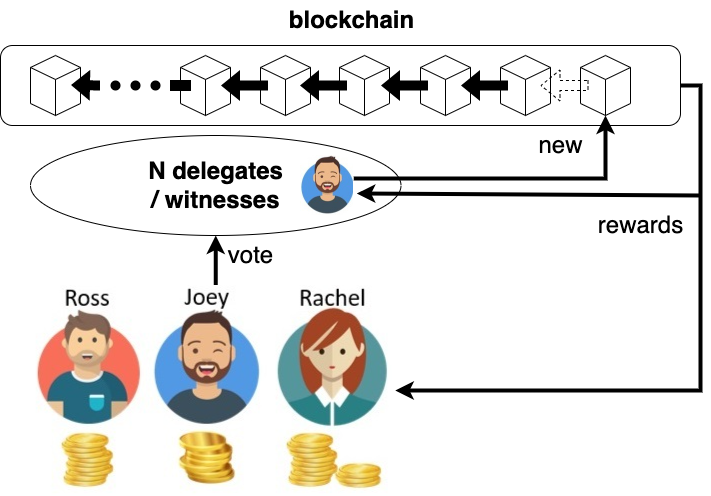
\includegraphics[scale=0.35]{img/DPoSKonzept.png}
	\caption{Konzept Delegated Proof of Stake\\Vgl. \cite{li2020comparison, nakuri} }
	\label{fig:konzept}
\end{figure}




\begin{table}
	\centering
	\begin{tabular}{lll}
		\toprule
		\textbf{Eigenschaft}       & \textbf{PoS}           & \textbf{DoS}
		\\\midrule
		\cell{Basis für                                                                \\Berechtigungsvergabe} &
		\cell{Größe des Stakes}    & \cell{Votes der                                   \\ Stakeholder}\\\\
		\cell{Throughtput                                                              \\ (Durchsatzmenge)}&
		\cell{Schnell}             & \cell{Sehr schnell}                               \\\\
		\cell{Dezentralität}       & \cell{Hoch}            & \cell{Gering}            \\\\
		\cell{Sicherheitsprobleme} & \cell{Matthew-Effekt}  & \cell{Angriffe durch     \\Delegierte}\\\\
		\cell{Belohnung}           & \cell{Ein Stakeholder} & \cell{Viele Stakeholder} \\\\
		\bottomrule
	\end{tabular}
	\caption{Gegenüberstellung\\Vgl. \cite{articleYang}}
	\label{tab:Vergleichs tabelle}
\end{table}

\begin{itemize}
	\setlength\itemsep{1.5em}
	\item Löst Probleme im Austausch für Dezentralität
	\item Keine generelle Verbesserung aber sinnvolle Erweiterung
	\item Auswahl von Konsensalgorithmus ist Anwendungsabhängig
\end{itemize}


\clearpage
\section{$CO_2$-Äquivalent Streaming und Nachrichten}
Streaming stützt sich auf eine komplexe Infrastruktur von Rechenzentren, Netzwerken und Geräten, die alle Strom verbrauchen und zu Kohlenstoffemissionen beitragen. Zu den wichtigsten Emissionsquellen gehören:
\begin{itemize}
	\item Datenzentren, die Inhalte speichern und verarbeiten
	\item Netzwerkinfrastruktur, die Daten überträgt
	\item Endverbrauchergeräte wie Fernseher, Computer und Smartphones
	\item Herstellung von Geräten und Infrastrukturkomponenten
\end{itemize}

Geschätzte CO2-Emissionen von Streaming-Medien:
\begin{itemize}
	\item Musik: 55 Gram per Stunde, ca. 7 Handy-Ladungen
	\item Video: 100 Gram pro Stunde (Netflix angaben), ca. 12 Handy-Ladungen
\end{itemize}
ABC News berichtet, dass der durchschnittliche Amerikaner jeden Tag 11 Stunden und 54 Minuten mit dem Internet verbringt.
Wenn eine Stunde Streaming etwa 100 Gramm CO2-Äquivalent entspricht und wir fast 12 Stunden am Tag streamen: 1.200 Gramm CO2-Äquivalent pro Tag~\cite{noauthor_is_nodate}.
Pro Jahr entspricht das 438 kg CO2-Äquivalent pro Person.
Bei 330 Millionen Amerikanern entspricht das 144,5 Millionen Tonnen CO2-Äquivalent pro Jahr.
Im Vergleich dazu: Die jährlichen CO2-Emissionen von Deutschland betragen 800 Millionen Tonnen.
\textbf{Diese Zahlen sind nur eine Schätzung und können je nach Quelle variieren.
	Falls wir sowas im Vortrag haben würde ich tiefer reingehen.}


Lösungen:
Die gemeinsame Nutzung von Peer-to-Peer (P2P) kann den CO2-Fußabdruck des Streamings durch kürzere Datenübertragungswege und effizientere Ressourcennutzung um 24-48\% verringern~\cite{8416363}.

\clearpage
\printbibliography


\end{document}